\chapter{Theoretical Background}
\label{chap:Theory}
Since 1930s, many theories and discoveries in particle physics have revealed the fundamental structure of matter. The matter is made up of fundamental particles and their interactions are mediated by four fundamental forces \cite{Griffiths:111880}. The theoretical models describe all the phenomena of particle physics as well as predict the nature and properties of particles. These models must be either confirmed experimentally or totally excluded giving hints of new physics. This interplay between experimental discoveries and the corresponding theoretical predictions leads to describe the fundamental particles and their interactions through a theoretical model, known as the Standard Model. The world's most powerful particle accelerators and detectors are used by physicists to test the predictions and limits of the Standard Model where it has successfully explained almost all experimental results. This chapter describes the Standard Model with the main focus on Quantum Chromodynamics and its properties which serve as the theoretical foundations of this thesis.

%The growing knowledge about fundamental and new particles was accompanied by the evolution of quantum mechanics and the special relativity. 
\section{Standard Model}
The Standard Model (SM) of particle physics \cite{Perkins:1982xb,Herrero:1998eq,Weinberg:1967tq} was developed in 1970s. It is a mathematical framework which describes the properties of fundamental particles and the forces of interactions between them, as summarized in Fig.~\ref{fig:SM}. According to the SM, there are 12 elementary particles i.e. without any internal structure, known as fermions. The fermions having half integral spin obeying Fermi-Dirac statistics and follows the Pauli exclusion principle. Each fermion has a corresponding antiparticle with same properties but opposite-sign quantum numbers.
\begin{figure}[!h]
\begin{center}
\hspace*{-15mm}
%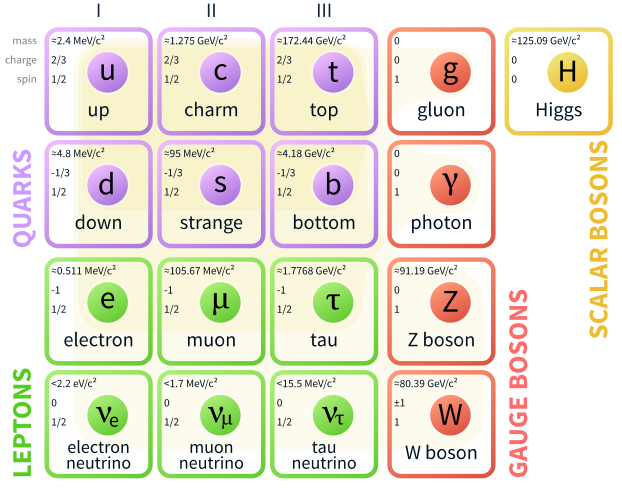
\includegraphics[scale = 0.8]{/home/anter/Desktop/Thesis/Figures/StandardModel_edited.png}\\
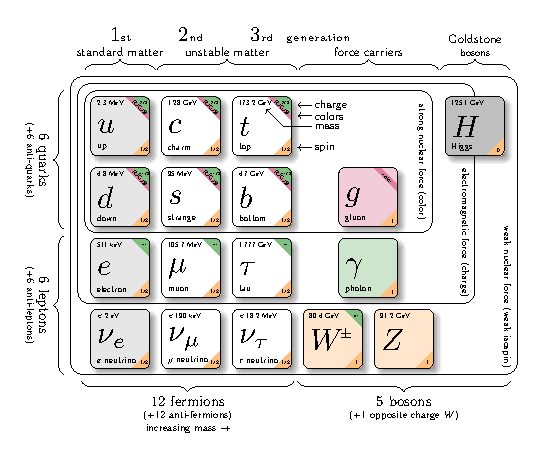
\includegraphics[width=1.2\textwidth]{/home/anter/Desktop/Thesis/Figures/model-physics.pdf}\\
%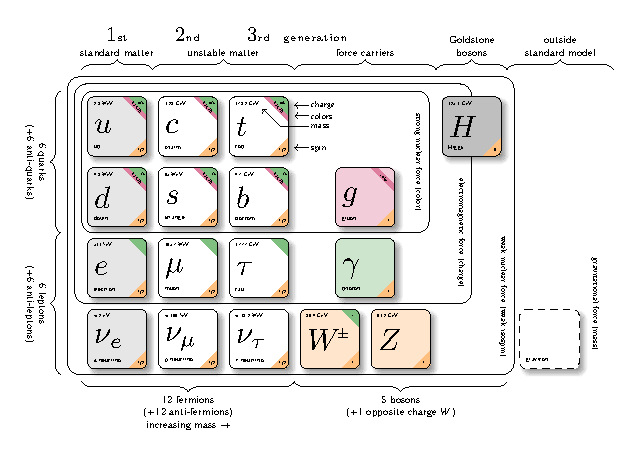
\includegraphics[width=1.2\textwidth]{/home/anter/Desktop/Thesis/Figures/original_model-physics.pdf}\\
\caption[The Standard Model summarizing the properties of elementary particles and their forces of interaction.]{The Standard Model\footnotemark summarizing the properties of elementary particles known as fermions (leptons and quarks), grouped into three generations, gauge bosons as mediators for the interactions, the scalar Higgs boson and not corporated graviton for the gravitational force.}
\label{fig:SM}
\end{center}
\end{figure}
\footnotetext{Source : \url{http://www.texample.net/tikz/examples/model-physics}}%https://en.wikipedia.org/wiki/Standard_Model}}
Depending on how the fermions interact, they are classified into two categories - leptons (\sln) and quarks ($q$). There are six types of leptons : electron ($e$), muon ($\mu$) and tau ($\tau$) with electric charge Q = -1 (all charges are in the units of elementary charge $e$) and the corresponding neutrinos $\nu_e$, $\nu_\mu$ and $\nu_\tau$ having electric charge Q = 0. There are six ``flavors'' of quarks : up ($u$), down ($d$), strange ($s$), charm ($c$), bottom ($b$) and top ($t$). $u$, $c$ and $t$ carry charge Q = $\pm$ $\frac{2}{3}$ whereas $d$, $s$ and $b$ carry charge Q = $\pm$ $\frac{1}{3}$. The quarks and leptons are categorized into three generations. The lightest and the most stable particles belong to first generation and the second and third generations have the heavier and less stable particles.

There are four fundamental forces existing in nature : electromagnetic, strong, weak and gravitational force. Every interaction involves the exchange of a gauge boson : the photon ($\gamma$) for the electromagnetic force, gluons ($g$) for the strong force, two $W$'s and a $Z$ for the weak force and the graviton (not yet found) for the gravitational force. However, the gravitational force has not been incorporated into SM yet. Along with this, the existence of dark matter or energy and the matter-antimatter asymmetry are still missing pieces in the SM. Each force acts between particles because of some property of that particle - charge for electromagnetism, color for the strong force and flavor for the weak force. 

In the SM, first three forces are unified into one quantum field theory \cite{Peskin:1995ev}, known as Grand Unified Theory (GUT) \cite{Glashow:1979pj,Salam:1980jd,Georgi:1974sy}. The SM framework is based on quantum field theories and is described by SU(3)$_{\rm C}~\otimes$ SU(2)$_{\rm L}~\otimes$ U(1)$_{\rm Y}$ gauge symmetry. Here, SU(2)$_{\rm L}~\otimes$ U(1)$_{\rm Y}$ term describes the weak and electromagnetic forces, respectively. The electromagnetic interaction of particles is explained by a well established modern theory of Quantum Electrodynamics (QED). In SM, the weak and electromagnetic interactions are combined by electroweak theory. The electroweak symmetry is spontaneously broken by the coupling to the scalar Higgs field. The gauge bosons of the unified electroweak theory are a mixture of the gauge bosons of the unbroken symmetry resulting in the massive $W^{\pm}$ and $Z$ bosons, and the massless photon ($\gamma$). The Higgs boson, named after Peter Higgs, is the field quantum of the Higgs field responsible for electroweak symmetry breaking. It was discovered by the CMS \cite{Chatrchyan:2012xdj} and ATLAS \cite{Aad:2012tfa} collaborations in 2012, with the properties consistent with the SM. The SU(3)$_{\rm C}$ term defines the strong interaction between quarks and gluons mediated by gluons, with the three degrees of freedom of the color charge (C). In contrast to the electroweak symmetry, the SU(3)$_{\rm C}$ of the strong interaction is an exact symmetry and hence the gluons are massless. The strong interaction between quarks and gluons is described by theory called Quantum Chromodynamics (QCD), explained in details in the next section of this thesis.

\section{Quantum Chromodynamics}
Quantum Chromodynamics \cite{Ellis:1991qj, Halzen:1984mc} is the non-abelian gauge theory of strong interactions between the quarks and gluons. The gauge group of QCD is the special unitary group SU(3)$_{\rm C}$ with color charges C as the generators of the gauge group. Color charge is the peculiar property of QCD and has a same role as the electric charge in electromagnetic interactions. However, the mediator of electromagnetic interactions i.e. photon, itself does not carry any electric charge where as the gluon carry color charge. This allows the self coupling of gluons and hence make the theory non-Abelian. Both the quarks and gluons carry three colors : red ($r$), green ($g$) and blue ($b$), and three anti-colors : anti-red ($\bar{r}$), anti-green ($\bar{g}$) and anti-blue ($\bar{b}$). The quarks carry a single color charge whereas gluons carry a combination of color charges. There are nine eigen states of gluons but one of them $\frac{1}{\sqrt{3}}(r\bar{r}~\plus g\bar{g}~\plus b\bar{b})$ is totally symmetric color singlet which has no net color charge and does not take part in interaction. The remaining eight eigen states of the gluons are :
\begin{equation}
r\bar{b},~r\bar{g},~b\bar{g},~b\bar{r},~g\bar{r},~g\bar{b},~\frac{1}{\sqrt{2}}(r\bar{r}~-~b\bar{b}),~\frac{1}{\sqrt{6}}(r\bar{r}~\plus b\bar{b}~-~2g\bar{g}) 
\end{equation}

The dynamics of the quarks and gluons are controlled by the gauge invariant QCD Lagrangian $\mathcal{L}_{QCD}$ which is composed of four terms as : 
\begin{equation}
\mathcal{L}_{QCD} = \underbrace{-\frac{1}{4}F^A_{\mu\nu}F^{\mu\nu}_A}_\text{$\mathcal{L}_{gluons}$}~\plus \underbrace{\sum\limits_{flavors}^{} \bar{q}_a \big(i\gamma^\mu (D_\mu)_{ab}~-~m_q\big)q_b}_\text{$\mathcal{L}_{quarks}$}~\plus \mathcal{L}_{gauge}~\plus\mathcal{L}_{ghost}
\label{eq:lag}
\end{equation}
where $\mathcal{L}_{gluons}$ represents the kinetic term of the gluon fields ${\cal A}^A_\mu$, $\mathcal{L}_{quarks}$ describes the interaction of spin-$\frac{1}{2}$ quark fields $q_a$ of mass $m_q$ with spin-1 gluon fields ${\cal A}^A_\mu$ summing over all presently known six flavors u, d, s, c, b, and t; $\mathcal{L}_{gauge}$ defines the chosen gauge and $\mathcal{L}_{ghost}$ is the so-called ghost term which is a remedy necessary to treat the degeneracy of equivalent gauge field configurations in non-Abelian gauge theories. Here the Greek letters $\mu$, $\nu$, ... $\in$ \{0,1,2,3\} represents space-time indices whereas a,b,c $\in$ \{1,2,3\} and A,B,C $\in$ \{1,...,8\} are the indices of the triplet and octet representations, respectively, of the SU(3)$_{\rm C}$ gauge symmetry group. $F^A_{\mu\nu}$ is the field tensor defined as
\begin{equation}
F^A_{\mu\nu} = \partial_\mu {\cal A}^A_\nu - \partial_\nu {\cal A}^A_\mu - g_s f_{ABC}{\cal A}^B_\mu {\cal A}^C_\nu
\label{eq:field}
\end{equation}
where $g_s$ is the coupling constant determining the strength of the interaction between colored partons and $f_{ABC}$ are the structure constants of the SU(3)$_{\rm C}$ group. The third term in Eq.~\ref{eq:field} is a non-Abelian term which distinguishes QCD from QED and gives rise to a three-gluon and a four-gluon vertex. ($D_\mu$)$_{ab}$ is the covariant derivative given by Eq.~\ref{eq:cov} and $\gamma_\mu$ are the Dirac $\gamma$-matrices. 
%In the second term of Eq.~\ref{eq:lag}, 
\begin{equation}
(D_\mu)_{ab} = \partial_{\mu}\delta_{ab}~\plus ig_sT^A_{ab}{\cal A}^A_\mu
\label{eq:cov}
\end{equation}
There are eight gluon fields ${\cal A}^A_\mu$ with factors $T^A_{ab}$ corresponding to the generators of the SU(3)$_{\rm C}$ gauge group. A representation of the generators is given via $T^A$ = $\lambda^A$/2 by the Hermitian and traceless Gell-Mann matrices $\lambda^A$ \cite{GellMann:1962xb}. The generator matrices $T^A$ satisfy the commutation relations 
\begin{equation}
\bigg[T^A,T^B\bigg] = if_{ABC}T^C
\end{equation}

In $\mathcal{L}_{QCD}$, the classical contribution comes from $\mathcal{L}_{gluons}$ and $\mathcal{L}_{quarks}$ terms which correspond to the free quark- and gluon-field terms, and the quark-gluon interaction term presented in Fig.~\ref{fig:feyn}. Along with this, the non-Abelian group structure of QCD leads to the cubic and quartic gluon self-interaction vertices, which are proportional to $g_s$ and $g^2_s$, respectively.

\begin{figure}[!h]
\begin{center}
\hspace*{-1mm}
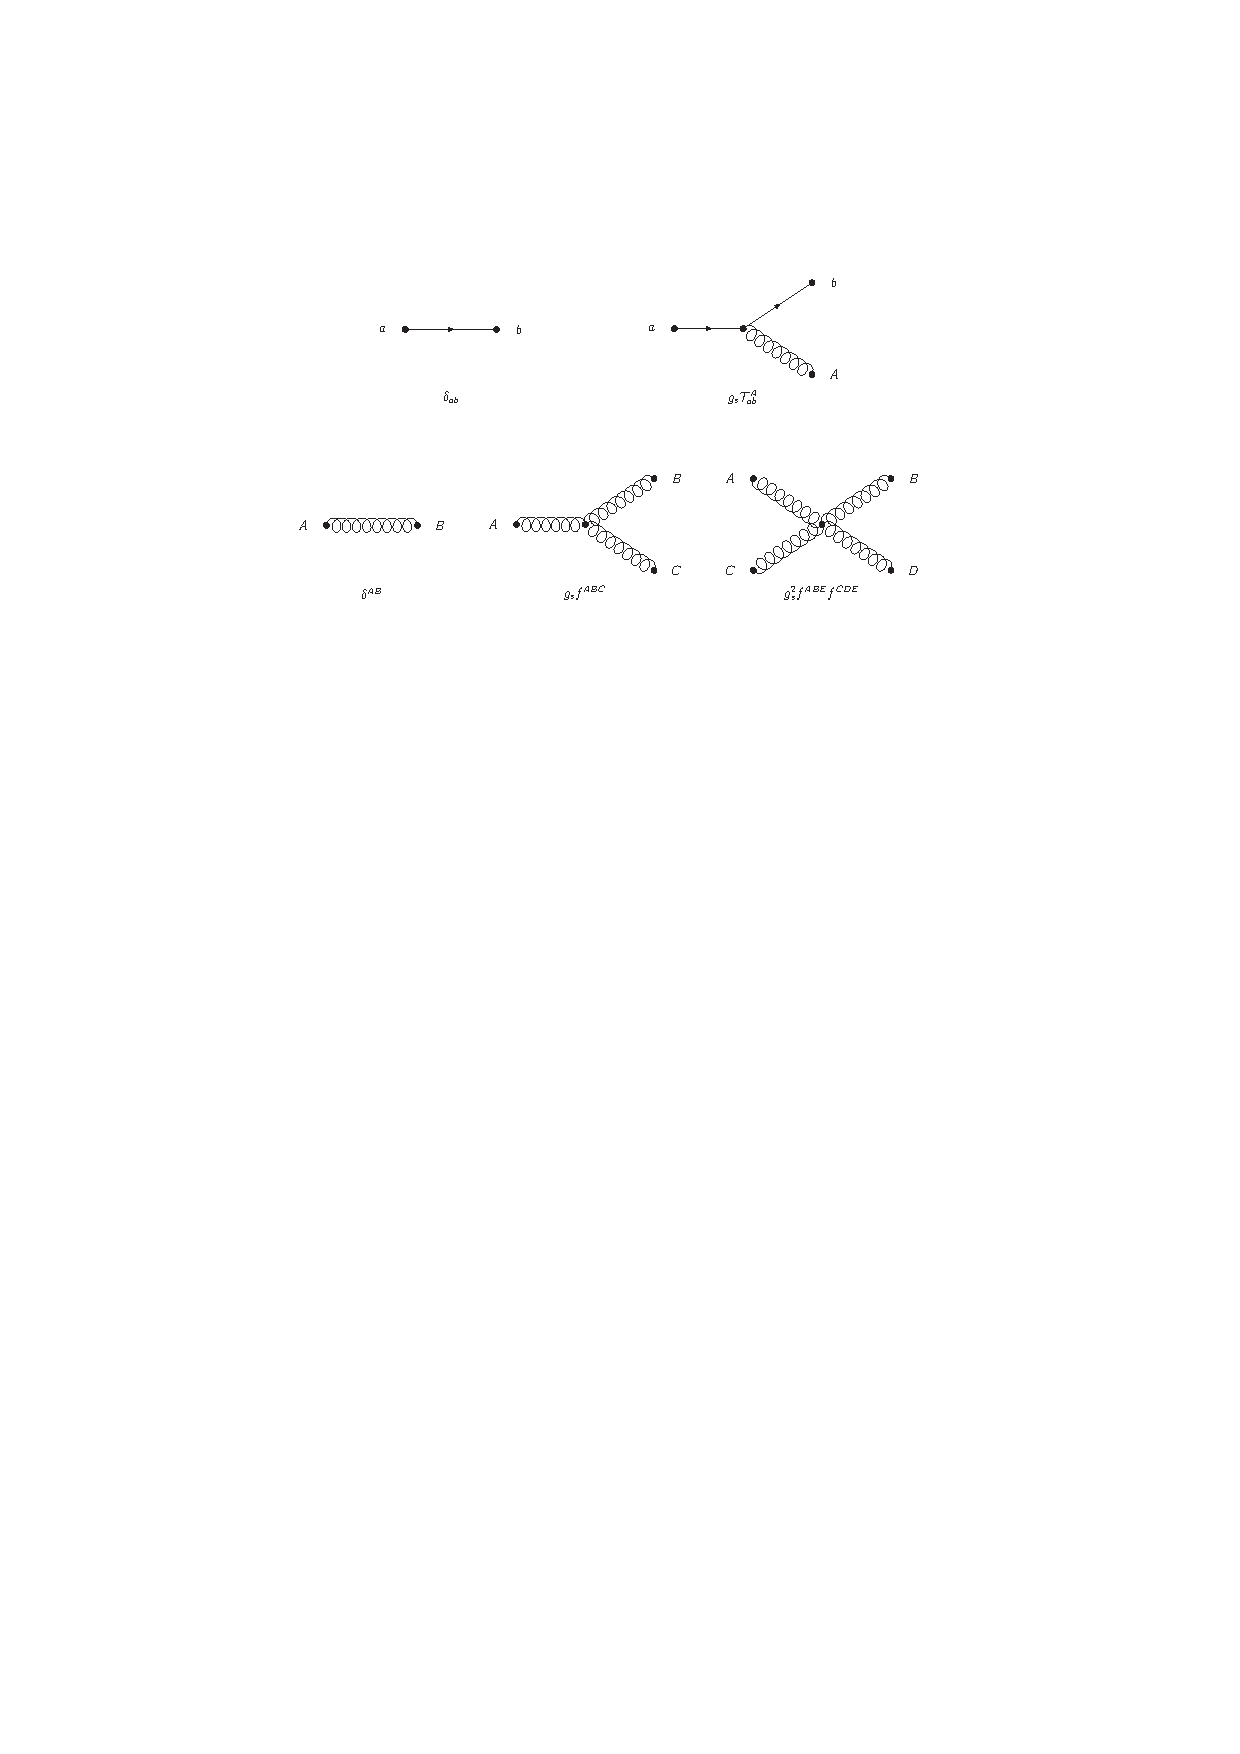
\includegraphics[width=0.95\textwidth]{/home/anter/Desktop/Thesis/Figures/edited_cropped_Feynmann.pdf}\\
\vspace*{4mm}
\caption[The fundamental Feynman rules of QCD.]{The fundamental Feynman rules of a free quark-field term (top left), quark-gluon interaction term (top right), free gluon-field term (bottom left), cubic gluon self-interaction term (bottom middle) and quartic gluon self-interaction term (bottom right). Taken from \cite{Rabbertz:2017ssq}.}
\label{fig:feyn}
\end{center}
\end{figure}

It is impossible to use perturbation theory on a gauge invariant Lagrangian without choosing a specific gauge in which to calculate. The usual gauge-fixing term is given by 
\begin{equation}
{\cal L}_{gauge}=-\frac{1}{2\xi} (\partial^{\mu}{\cal A}^{A}_{\mu})^{2}
\label{eq:gauge-fixing}
\end{equation}
where $\xi$ may be any finite constant. This choice fixes the class of covariant gauges with $\xi$ as the gauge parameter. As QCD is non-Abelian, the gauge fixing term must be supplemented by a ghost Lagrangian as
\begin{equation}
{\cal L}_{ghost}=\partial_{\alpha}\eta^{A\dagger}(D^{\mu}_{AB}\eta^{B})
\label{eq:ghost}
\end{equation}
where $\eta^{A}$ is a complex scalar field which obeys Fermi statistics. The ghost fields cancel unphysical degrees of freedom which arise due to using covariant gauges. This completes the QCD Lagrangian shown in Eq.~\ref{eq:lag}.

The strength of an interaction is given by a fundamental parameter called the coupling constant $\alpha$. In QED, the coupling constant $\alpha_e$ = $e^2/4\pi$ = 1/137 is constant. In contrast to this, in QCD, the coupling constant \alpsq = $g^2_s/4\pi$ is not constant and depends on the separation between the interacting particles. It increases with the increase in the distance or decrease in the energy scale Q. At large distances or low energies, the quarks can never be found as free particles but as color neutral bound states called hadrons. Hadrons are of two types : baryons and mesons made up of quark-antiquark pair and ($qqq$) made from three (anti-)quarks. According to the quark model \cite{Griffiths:111880} every (anti-)baryon is made up of three (anti-)quarks and every meson is composed of a quark and an antiquark. When the colored quarks and gluons within a hadron are pulled farther and farther apart, there is an increase in the strength of force between them. This results in creation of new quark-antiquark pair making difficult to liberate a free quark or gluon. This property of QCD is known as confinement. As it would take an infinite amount of energy to separate two quarks, they are forever bound into hadrons such as protons ($uud$), neutrons ($udd$). Although the gluons are massless, the confinement leads to the finite range of the strong interactions. On the other hand, at small distances, the quarks and gluons interact very weakly and are treated as free particles. This property is known as asymptotic freedom. This indicates that perturbation theory is only applicable at high energies or small distances.

\subsection{Perturbative Quantum Chromodynamics}
At high energies, the property of asymptotic freedom allows a perturbative treatment in QCD calculations. In perturbative Quantum Chromodynamics (pQCD), any observable $X$ such as cross-section of a scattering process, can be written as a perturbative series in terms of coupling constant \alps as : 
\begin{equation}
X = \sum\limits_{i=0}^{N} \alpha^n_s {\rm c}_i = {\rm c}_0~\plus \alpha^1_s {\rm c}_1~\plus \alpha^2_s {\rm c}_2~\plus ...
\end{equation} 
where ${\rm c}_i$ are the perturbative coefficients. In a process, the pQCD calculation of X is determined by over the amplitudes of all Feynman diagrams. For a given Feynman diagram, the power of \alps is determined by the number of vertices associated with quark-gluon or gluon-gluon interactions. A leading order (LO) prediction sums over only the lowest-order contribution whereas next-to-leading order (NLO) includes terms with an additional powers of \alps. The next-next-to-leading order (NNLO) includes emission of another gluon or a virtual gluon loop. The different order of the QCD processes are shown in Fig.~\ref{fig:orders}.
\begin{figure}[!h]
\begin{center}
\hspace*{-1mm}
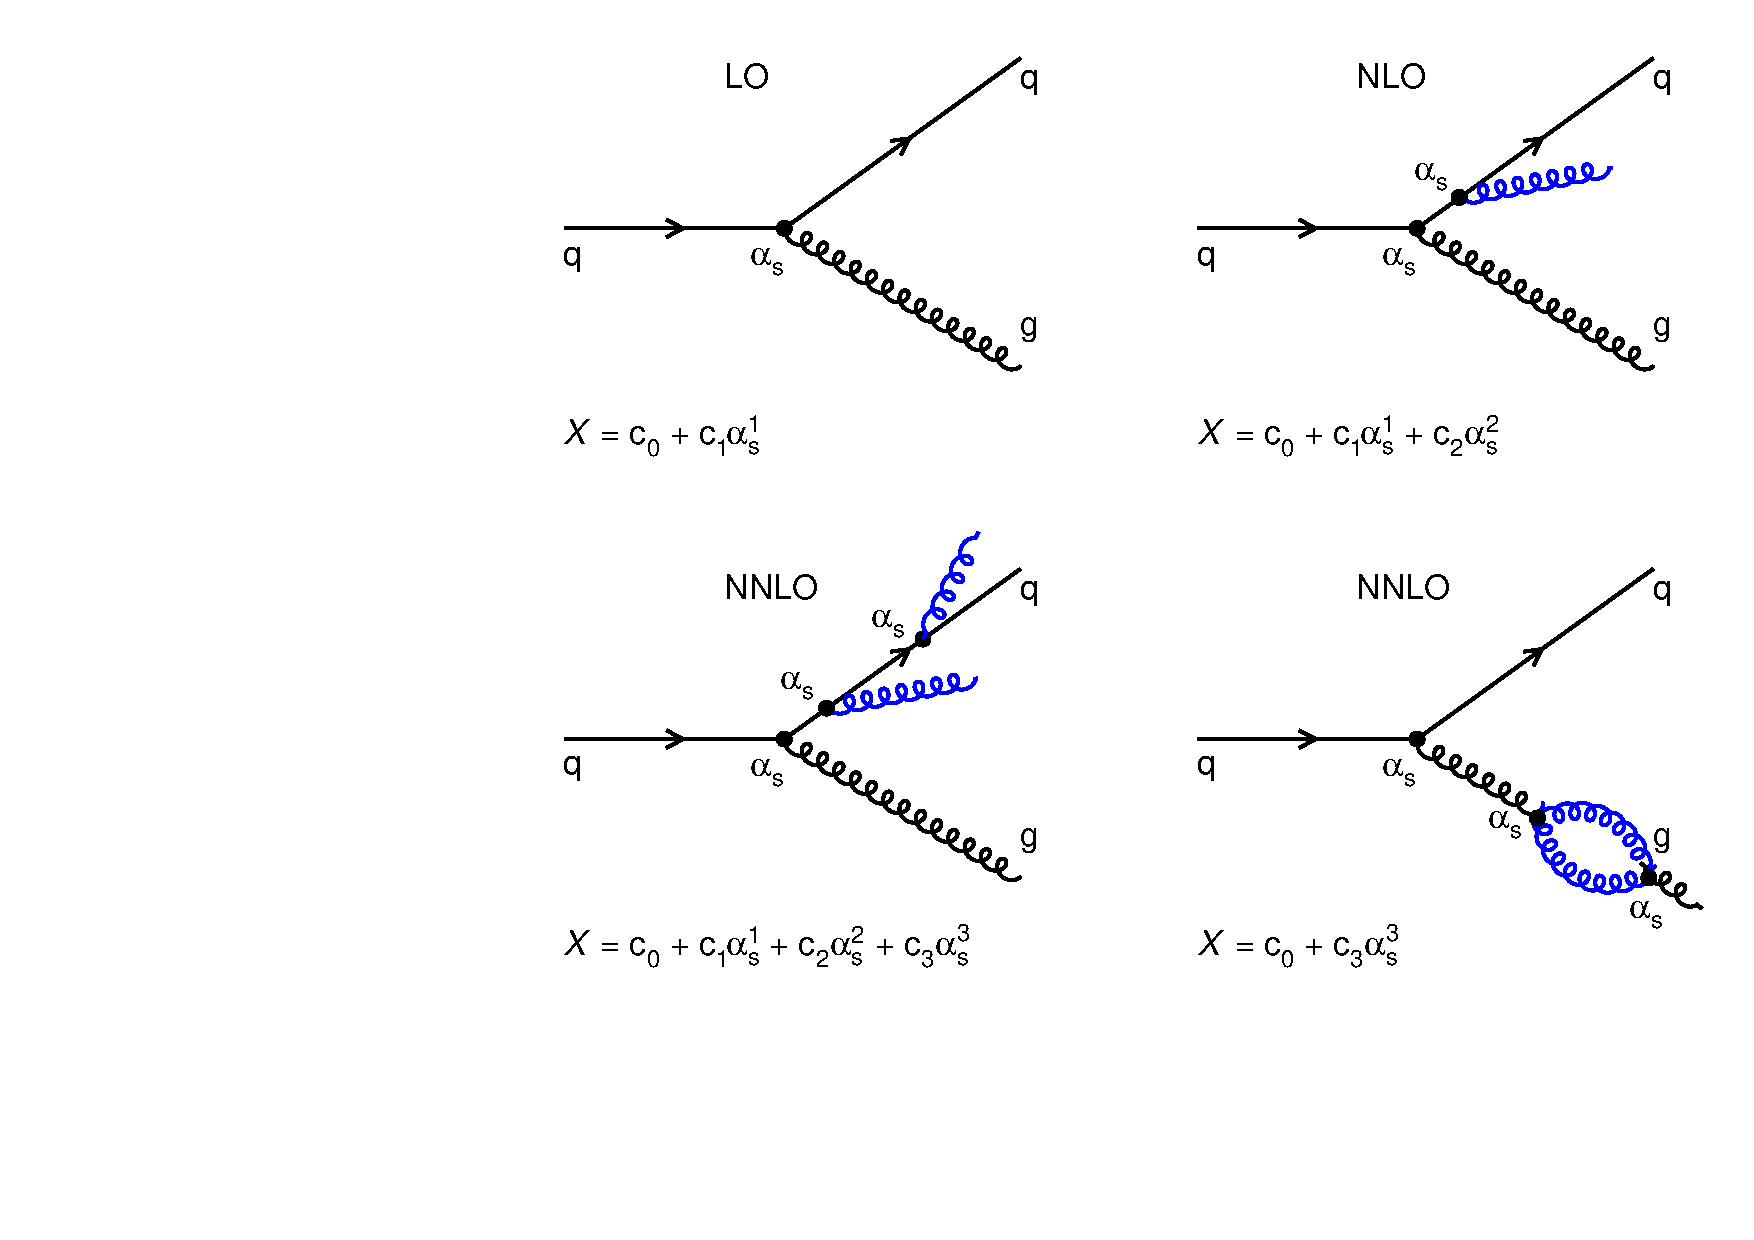
\includegraphics[width=0.95\textwidth]{/home/anter/Desktop/Thesis/Figures/Orders.pdf}\\
\vspace*{4mm}
\caption[Feynman diagrams showing leading-order (LO), next-to-leading order (NLO) and next-next-to-leading order (NNLO) processes in QCD.]{Feynman diagrams\footnotemark showing leading-order (LO), next-to-leading order (NLO) and next-next-to-leading order (NNLO) processes in QCD along with the perturbative expansion of any observable $X$ in powers of the strong coupling constant \alps. At each successive step in perturbation series, the emission of an additional gluon take place.}
\label{fig:orders}
\end{center}
\end{figure}
The calculations become complex with the loop diagrams where the momenta of the virtual particles in a loop are not fully constrained by four-momentum conservation and the associated integrals are divergent. Such ultraviolet (UV) divergencies enter the calculations beyond LO due to loop or vertex corrections. These are overcome by a procedure known as renormalization, described in next Section. Apart from these, QCD also suffers from infrared and collinear divergences (IRC) due to the presence of massless gluons and neglected quark masses. These need to be handled in pQCD calculations. The observable to be studied must be IRC safe. 

\subsection{Renormalization and Running of the Strong Coupling}
The renormalization is a mathematical procedure which allows the finite calculation of momenta integrals of loop by removing UV divergences. \footnotetext{Drawn using ROOT}It introduces a regulator for the infinities, the renormalization scale \mur. At first, the divergences are regularized temporarily by introducing a cut-off to the loop momenta at \mur scale. Then the free parameters of the Lagrangian, i.e. the coupling constant are redefined (renormalized) to absorb the UV divergences. Hence, both \alpsq and observable $X$ become a function of \mur. The exact dependence of \alpsmusq on \mur is described by the renormalization group equation (RGE), which determines the running of \alpsmusq. RGE states that the dependence of $X$ on \mur must cancel, which is expressed mathematically as : 
\begin{equation}
\mur^{2}\frac{d}{d\mur^{2}}X\Bigg(\frac{Q^{2}}{\mur^{2}},\alpha_{s}(\mur^{2})\Bigg)=
\Bigg(\mur^{2}\frac{\partial}{\partial\mur^{2}}~\plus \mur^{2}\frac{\partial\alpha_{s}(\mur^{2})}
{\partial\mur^{2}}\frac{\partial}{\partial\alpha_{s}(\mur^{2})}\Bigg)X=0
\label{eq:dmu}
\end{equation}
Using $\beta(\alps)$ = $\mur^{2}\frac{\partial\alpha_{s}(\mur^{2})}{\partial\mur^{2}}$, Eq.~\ref{eq:dmu} can be re-written as 
\begin{equation}
\Bigg(\mur^{2}\frac{\partial}{\partial\mur^{2}}~\plus \beta(\alps)\frac{\partial}{\partial\alpha_{s}(\mur^{2})}\Bigg)X=0
\label{eq:dmu2}
\end{equation}
By setting the renormalization scale to the physical scale i.e. $Q^{2}=\mu^{2}$, $X(1,\alpha_{s}(Q))$ is a solution to above equation. $Q$-dependence of the $X$ is only from the renormalization of the theory and would not be present in the classical theory. Hence measuring the $Q$-dependence of $X$ will directly probe the quantum structure of the theory. The $\beta$ function in QCD has a perturbative expansion as : 
\begin{equation}
\beta(\alps)=-\alpha_{s}^{2}\Big(b_0~\plus b_1\alps~\plus b_2\alpha_{s}^{2}~\plus {\cal O}(\alpha_{s}^{3})\Big) 
\label{eq:beta}
\end{equation}
where $b_0$, $b_1$ and $b_2$ are the 1-loop, 2-loop and 3-loop $\beta$-function coefficients encoding the dependence of the coupling on the energy scale and given in the modified minimal subtraction ($\overline{\rm MS}$) scheme \cite{tHooft:1973mfk,Weinberg:1951ss} as :
\begin{equation}
b_0 = \frac{33-2n_f}{12\pi}, ~~~b_1 = \frac{153-19n_f}{24\pi^2}, ~~b_2 = \frac{77139 - 15099n_f~\plus 325n^2_f}{3456\pi^3}
\end{equation}
where $n_f$ is the number of quark flavours with masses $m_q$ smaller than the scale \mur. On integration of above equation, the energy dependence of \alps is yielded. Neglecting the higher orders, the first order solution of RGE is :
\begin{equation}
\alpha_{s}(\mur^2)=\frac{1}{b_0~{\rm ln}(\mur^2/\Lambda^2_{QCD})}
\label{eq:sol}
\end{equation}
with $\Lambda_{QCD}$ as the constant of integration. It corresponds to the scale at which the perturbative coupling would become large and the perturbative series diverge. With $b_0$ \gr 0, the coupling becomes weaker at higher scales $Q$, i.e. the effective color charge gets smaller when the distance decreases. This allows the quarks to behave as free particles within the hadron, leading to the property called asymptotic freedom. It is convenient to express \alps at some fixed scale. As some of the best measurements come from $Z^0$ decays, it is common practise to give the strong coupling at the scale of the $Z$ boson mass as \alpsmz. So, Eq.~\ref{eq:sol} can be expressed as :
\begin{equation}
\alps\big(\mur,\alpsmz\big) = \frac{\alpsmz}{1\plus\alpsmz b_0{\rm ln}(\mur^2/M^2_z)}
\end{equation}

The free parameter \alps of the theory is deduced from experimental measurements and evolved to the scale of the $Z$ boson. The current world average value of the strong coupling constant according to the PDG \cite{Patrignani:2016xqp} is 
\begin{equation}
\alpsmz = 0.1181 \pm 0.0011
\end{equation}
This value is derived using hadronic $\tau$ lepton decays, lattice QCD calculations, deep inelastic scattering data, electron-positron annihilation processes and electroweak precision fits. The various determinations of the strong coupling constant at scale $Q$, describing the running of the strong coupling up to the 1 TeV scale, are shown in Fig.~\ref{fig:alpha_pdg}.

\begin{figure}[!h]
\begin{center}
\hspace*{-7mm}
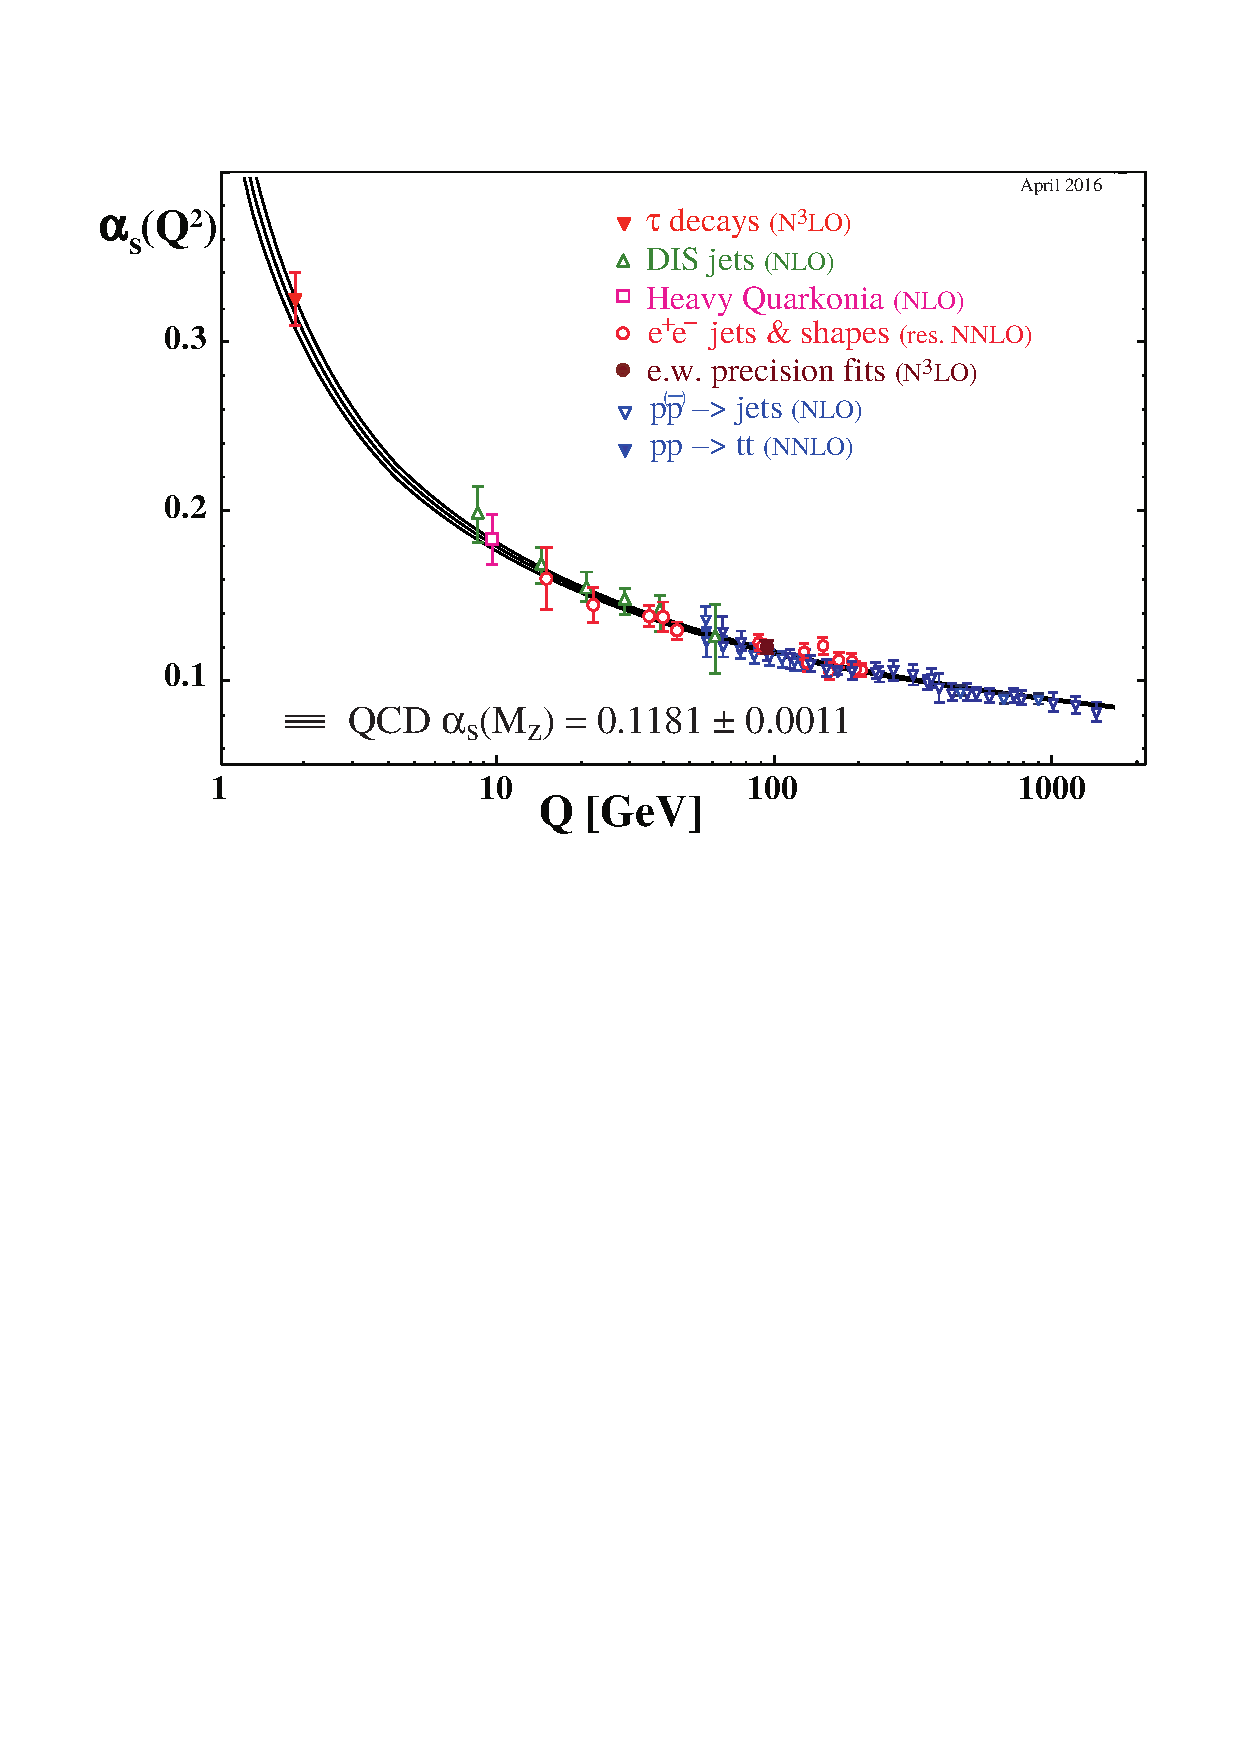
\includegraphics[width=0.95\textwidth]{/home/anter/Desktop/Thesis/Figures/cropped_Alpha.pdf}\\
\vspace*{4mm}
\caption[Running of the strong coupling constant.]{The measurement of the strong coupling constant \alps as a function of the energy scale $Q$ from various experiments is are shown. These describe the running of the \alps up to the 1 TeV scale. Taken from ~\cite{Patrignani:2016xqp}.}
\label{fig:alpha_pdg}
\end{center}
\end{figure}

\section{Hadronic Collisions}

The collision between two hadrons is visualized as an interaction between their constituents, known as partons - quarks and gluons, at at a large momentum transfer, $Q$. At the Large Hadron Collider (LHC), the hadrons involved in the collisions are protons : a complex composite particles consisting of three valence quarks ($uud$) and gluons for the exchange of the strong force. The proton also contains `sea quarks' consisting of quark-anti-quark pairs coming into and out of existence rapidly and continuously due to gluon colour field splitting. In a collision, one of the most important quantities to evaluate is the cross-section ($\sigma$) of a certain process. It gives the probability that the two hadrons interact and give rise to that specific process. But in a hadronic collision, the perturbation theory is only valid at the parton-level and due to property of confinement at low energies, free partons cannot exist in nature. Only hadrons having a complex internal structure are available for the high energy collisions. So, a factorization theorem of QCD \cite{Collins:1989gx} comes into play which allows the calculation of $\sigma$ by separating into two parts : a short-distance partonic cross-section calculable with pQCD, and a non-perturbative long-distance part described by parton distribution functions (PDFs) $f_i(x,\muf)$. \muf is a factorization scale which corresponds to the resolution with which the hadron is being probed. The particles emitted with transverse momenta above \muf are considered in the hard scattering perturbative coefficients whereas those emitted with transverse momenta less than \muf are accounted for within the PDFs. The PDFs describe the partonic content of the colliding hadrons and give the probability to find a parton $i$ with momentum fraction $x$ within a hadron $h$. Assuming factorization theorem in a proton-proton collision, the cross-section of a hard scattering process can be written as :
\begin{equation}
\begin{gathered}
\sigma_{P_1P_2 \rightarrow X} = \sum\limits_{i,j}^{}\int_{}^{} dx_1dx_2f_{i,P_1}(x_1,\muf)f_{j,P_2}(x_2,\muf)\\\times~\hat\sigma_{ij\rightarrow X} \Bigg(x_1p_1,x_2p_2,\alpha(\mur^2),\frac{Q^2}{\muf^2}\Bigg)
\end{gathered}
\end{equation}
where $i,~j$ are initial-state parton flavours, $f_i$ and $f_{j}$ are the proton PDFs which depend on momentum fractions $x_1$ and $x_2$ of parent protons $P_1$ and $P_2$ respectively as well as on the factorization scale \muf. The sum extends over all contributing initial-state partons. $\hat\sigma_{ij}$ is parton level cross-section for the production of final state $X$ and depends on the final state phase, the factorization scale \muf and the renormalization scale \mur. The schematic illustration of the factorization into the PDFs and the hard scattering cross-section is presented in Fig.~\ref{fig:fac}.
\begin{figure}[!h]
\begin{center}
\hspace*{-7mm}
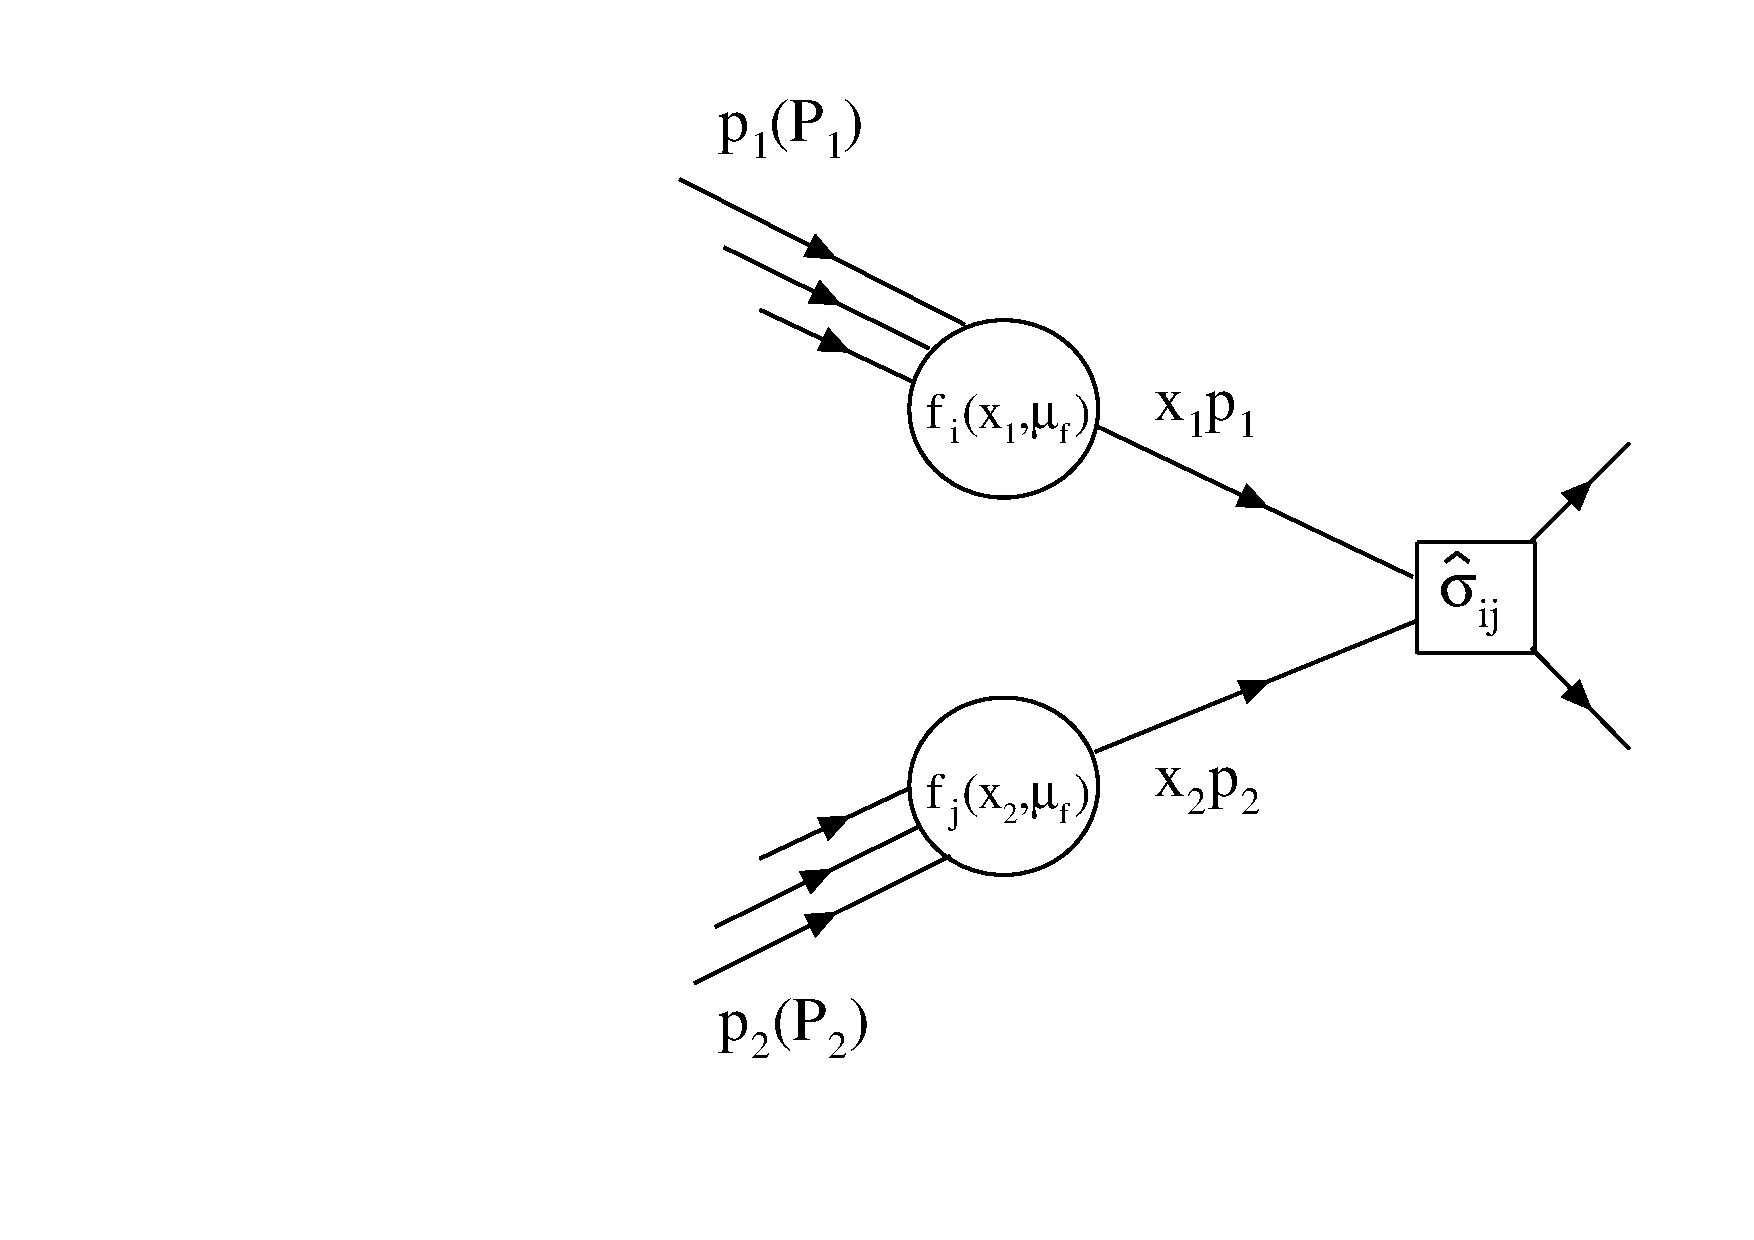
\includegraphics[width=0.65\textwidth]{/home/anter/Desktop/Thesis/Figures/Factorization.pdf}\\
\vspace*{4mm}
\caption[Schematic illustration of factorization theorem in a collision of two hadrons (protons here).]{Schematic illustration\footnotemark~of factorization theorem in a collision of two hadrons (protons here) leading to a hard-scattering process at a scale $Q^2$. The two partons $x_1$ and $x_2$ participate in hard interaction with momenta $x_1p_1$ and $x_2p_2$, where $p_1$ and $p_2$ are the momenta of the colliding protons $P_1$ and $P_2$, respectively. The total cross-section is factorized into the hard scattering cross-section $\hat\sigma_{ij}$ calculable using perturbative Quantum Chromodynamics and the PDFs $f_i(x_1,\muf)$ and $f_j(x_2,\muf)$ with factorization scale \muf.}
\label{fig:fac}
\end{center}
\end{figure}
The PDFs of the proton are a necessary input to almost all theory predictions for the hadron colliders. The QCD does not predict the parton content of the proton. So the shapes of PDFs are determined in fits to experimental measurements from data of different experiments. The dependence of PDFs on \muf is calculated using the Dokshitzer-Gribov-Lipatov-Altarelli-Parisi (DGLAP) \cite{Gribov:1972ri,Dokshitzer:1977sg,Altarelli:1977zs} equations which use \alps and the RGE as inputs. The knowledge of proton PDFs mainly comes from the Deep Inelastic Scattering (DIS) HERA, fixed target and TEVATRON data. The LHC data has a potential to improve constraints of the PDFs further as done in one of the recent measurements \cite{Sirunyan:2017skj}. There are several groups which determine the PDFs with the differences in the applied minimization method, the phenomenological approaches and the estimation of the uncertainties. The global PDFs are the CTEQ \cite{Dulat:2015mca}, MMHT \cite{Harland-Lang:2014zoa}, NNPDF \cite{Ball:2014uwa}, ABM \cite{Alekhin:2012ig} and HERAPDF \cite{Abramowicz:2015mha} groups at LO, NLO and NNLO.
\footnotetext{Drawn using ROOT}%Source : \url{https://arxiv.org/pdf/1003.0521.pdf}}

\subsection{Parton Shower and Hadronization}
The hard scattering process involves large momentum transfers due to which the partons involved in it get accelerated. These accelerated colored partons emit QCD radiation in the form of gluons with successively lower energy. Unlike the uncharged photons in QED, the gluons themselves carry color charge and hence also emit further gluons. The emitted gluons in turn splits into $q\bar{q}$ pairs. This leads to a shower of colored partons called the parton shower. The collinear parton splitting described by splitting functions and the soft gluon emissions contribute mainly to parton shower. The parton shower mimics the effect of higher-order corrections to the hard process. These cannot be calculated exactly and are taken into account using the parton shower approximation. The two incoming partons which are constituents of two colliding hadrons can also develop parton showers, commonly known as Initial-State Radiation (ISR). The initial parton showers till they collide to initiate the hard scattering process. The final outgoing partons produced from a hard scattering process undergo parton showering and give rise to Final-State Radiation (FSR). A parton shower terminates when the scale is below the hadronization scale, which is of order 1 GeV.

With the decrease in energy of partons, the coupling constant of QCD \alps evolves and become large. This leads to the confinement of colored quarks and gluons which leads to the formation of color-neutral composite particles called hadrons. This process is known as hadronization. This process takes place at low momentum transfer and hence non-perturbative in nature. Although no exact theory for hadronization is known, the different phenomenological models have been developed to explain the process of hadronization. These are implemented in Monte Carlo event generators to simulate the hadronization process. \PYTHIA~uses the Lund string model while \HERWIG~is based on the cluster fragmentation model. \\\newline
{\bf Lund String Model -} In the Lund string model of hadronization \cite{Andersson:1998tv}, the highest-energy gluons are treated as field lines. Due to the gluon self-interaction, the gluons are attracted to each other and form a narrow tube (or string) of strong color field between a $q\bar{q}$ pair. This model is based on an observation that at distances greater than about a femtometer, the potential energy $V(r)$ of colored quarks grows linearly with the increase in distance between them ($r$) as :
\begin{equation}
V(r) = \kappa r
\end{equation}
where $\kappa \sim {\rm GeV/fm^2}$ is the tension of the string connecting the quarks. When the $q$ and $\bar{q}$ move apart, the gluonic string gets stretched between them and its potential energy grows at the expense of their kinetic energy. When the potential energy becomes of the order of hadron masses, the potential energy is so large that the string breaks at some point along its length, creating a new $q\bar{q}$ pair. The two string segments then again stretch and break until all the potential energy gets converted to $q\bar{q}$ pairs. this whole process is illustrated in Fig~\ref{fig:string}. Then $q$ and $\bar{q}$ hadronize into hadrons due to confinement property. \\ \newline
{\bf Cluster Model -} The cluster model of hadronization \cite{Marchesini:1987cf,Webber:1983if} is based on preconfinement property of QCD \cite{Amati:1979fg}. According to this property, at evolution scales $Q_0$ much less than the hard process scale $Q$, the partons in a shower are clustered in colourless groups with an invariant mass distribution, depending on $Q_0$, not on $Q$ and nature of hard process. This model contains two steps : firstly all gluons split into $q\bar{q}$ pairs at the end of the parton shower and in the second step, a new set of low-mass color-singlet clusters are obtained which decay into either secondary clusters or directly into hadrons. However, this model has problems in dealing with the decay of very massive clusters.

\begin{figure}[!h]
\begin{center}
\hspace*{-4mm}
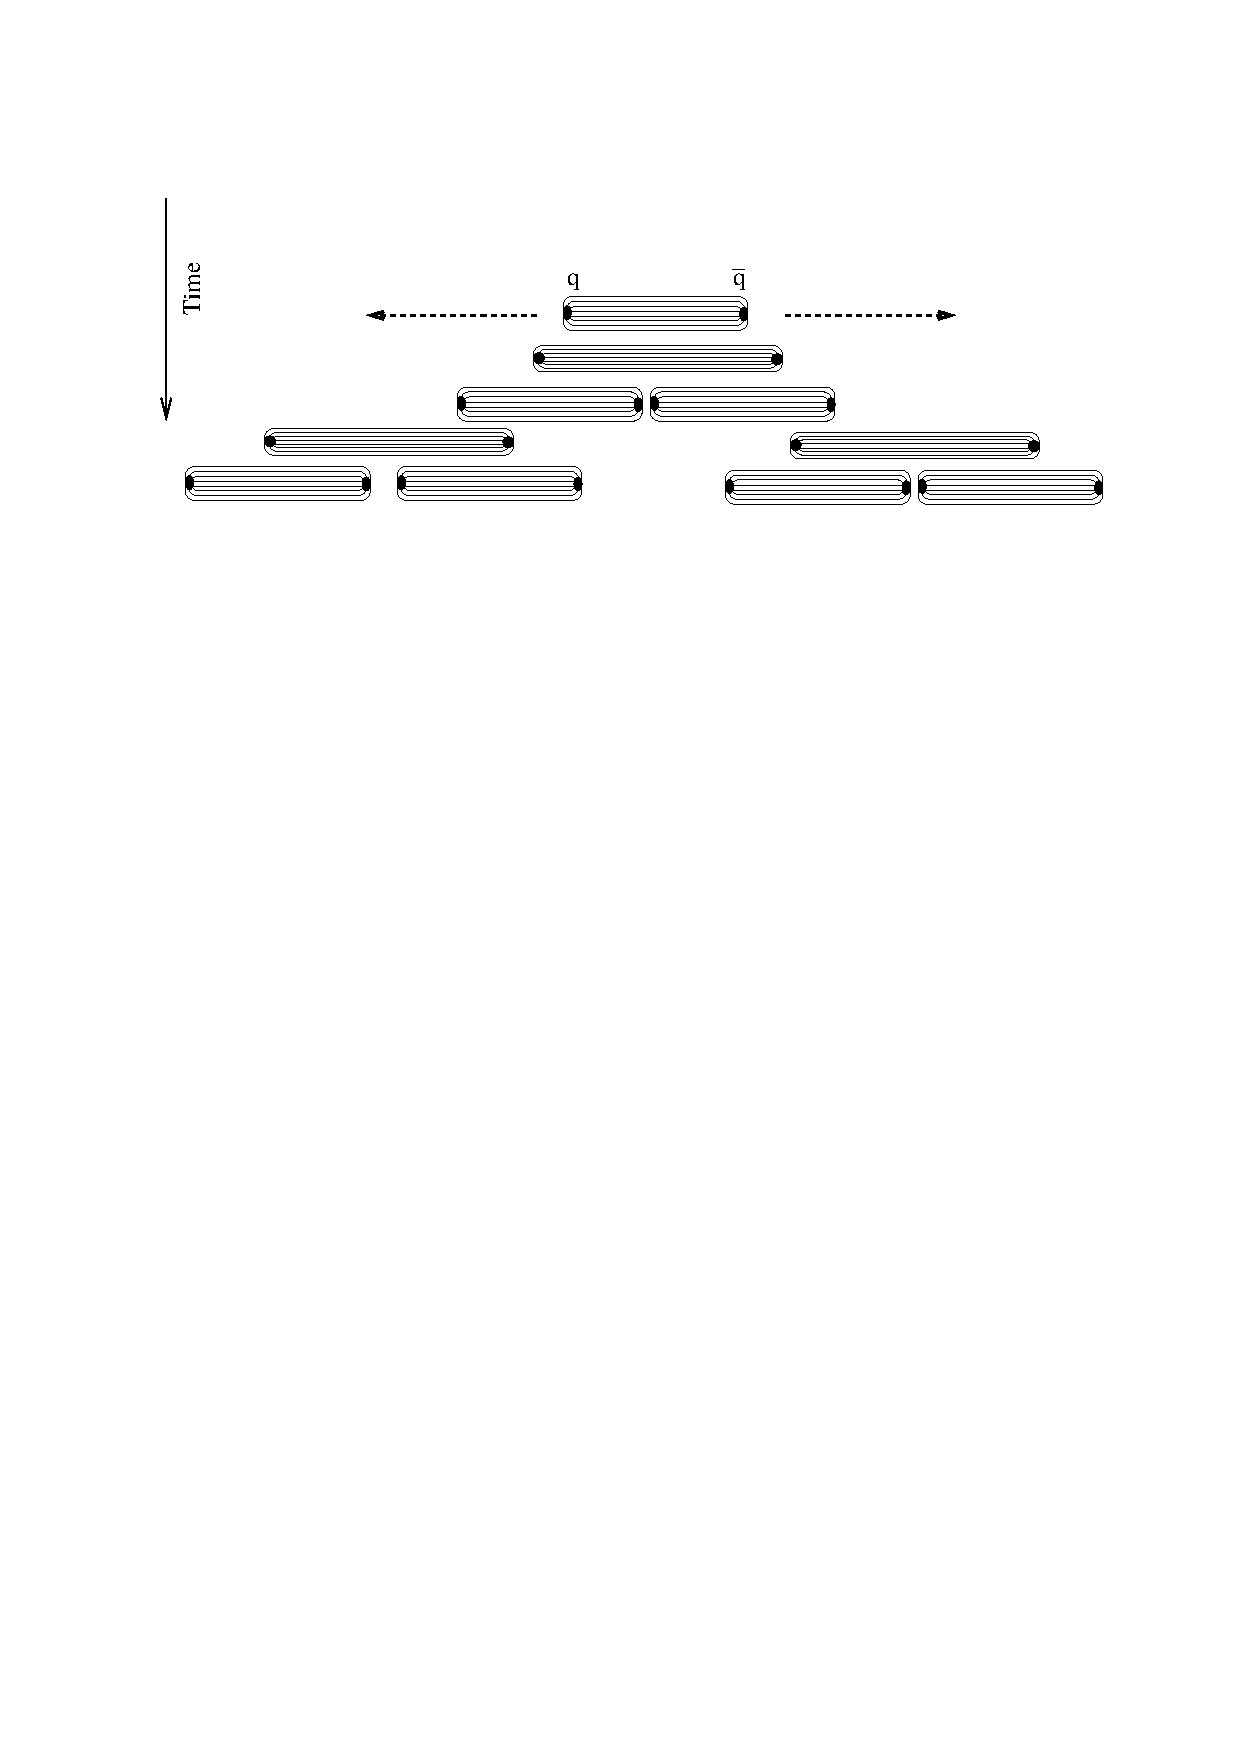
\includegraphics[width=0.95\textwidth]{/home/anter/Desktop/Thesis/Figures/cropped_String.pdf}\\
\vspace*{4mm}
\caption[Illustration of the hadronization process in Lund string model.]{Illustration of the hadronization process in Lund string model\footnotemark. As the quark $q$ and anti-quark $\bar{q}$ move apart, the potential energy of the gluonic string increases. When it becomes of the order of hadron masses, the string breaks and a new $q\bar{q}$ pair is created. The breaking of string and creation of $q\bar{q}$ continues till all the potential energy gets converted to $q\bar{q}$ pairs which then get hadronized.}
\label{fig:string}
\end{center}
\end{figure}

\subsection{Underlying Event}
In a high energy proton-proton collisions, the underlying event (UE) includes the effects which are not coming from the primary hard scattering process. The UE include the contributions from relatively small momentum transfer processes : initial and final-state radiations (ISR, FSR), leftover partons in the collisions called beam remnants and multiple parton interactions (MPI). Due to composite nature of proton, the remaining two partons which do not participate in a hard collision may also interact giving rise to multiple parton interactions. The UE induces an additional energy in the detector which is not related to the main hard interaction. This acts an unavoidable background which needs to be removed. Hence, it is very crucial to study and understand the UE. The UE activity increases with $Q$ and the center-of-mass energy \cme. Figure~\ref{fig:MPI} shows the complex variety of processes taking place in a single proton-proton collision.
\footnotetext{Source : \url{http://inspirehep.net/record/806744}}

\begin{figure}[!h]
\begin{center}
\hspace*{-7mm}
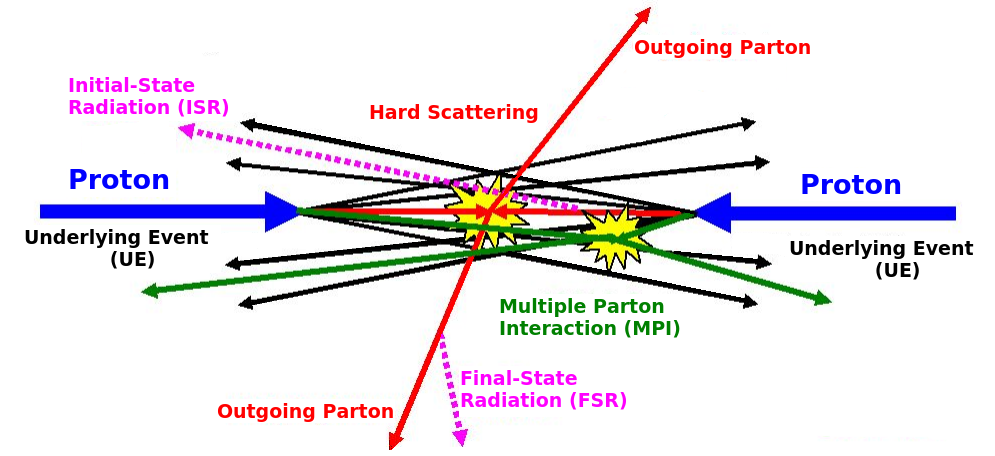
\includegraphics[width=0.95\textwidth]{/home/anter/Desktop/Thesis/Figures/MPI.png}\\
\vspace*{4mm}
\caption[Proton-proton collision.]{A proton-proton collision involving the hard scattering process, along with initial- and final-state radiation (ISR and FSR) complemented with multiple parton interactions (MPI) and collisions from leftover partons called beam remnants. All these processes with low momentum transfer contribute to underlying event (UE)\footnotemark.}
\label{fig:MPI}
\end{center}
\end{figure}

The bunch of hadrons, produced from hadronization of quarks and gluons, gets collimated towards the direction of the initial parton that originated them, in the form of ``jets''. The jets, being the final structures observed experimentally in detectors, act as a bridge between the elementary quarks and gluons of QCD and the final hadrons produced in high energy collisions. Therefore, at large momentum transfer of the interacting partons, jets and their observables are the best tools to test the predictions of pQCD. Also, the jet production is sensitive to the strong coupling constant \alpsns. The precise knowledge of the jet cross-section can help to extract the value of \alps and also to reduce the uncertainties of the PDFs of proton. In LHC, the simplest jet production process is 2 $\rightarrow$ 2 scattering process at leading-order giving dijet events. But the partons coming from ISR, FSR or MPI can also hadronize to produce jets greater than 2 in a single proton-proton collision, resulting in multijet events. The investigation of inclusive multijet event cross-sections permits more elaborate tests of QCD. Also, a precise understanding of jet variables is an essential to understand the signal and background modelling for the new physics search in hadronic final states. In this thesis, the multijet production cross-sections are exploited to extract the value of strong coupling constant \alps. In the next section, we focus on the definition of a jet.
\footnotetext{Source : \href{https://www-cdf.fnal.gov/physics/new/qcd/ue_escan/}{The Energy Dependence of Min-Bias and the Underlying Event at CDF}}
\section{Jets}
\label{sec:jets}
Jets \cite{Sterman:1977wj} are the conical structures which group the hadrons into a single physics entity. The first evidence for a jet structure was found in hadron production of $e^\plus e^-$ annihilation at SLAC in 1975 \cite{Hanson:1975fe}. Since the partons can not exist as free particles and therefore can not be measured directly by the experiments. The information about the dynamics of the partons can be obtained from jets because the configurations of high-energy quarks and gluons at short distances are truly reflected in the energy and angular distributions of the jets. The clustering of particles is performed by applying jet algorithms.

\subsection{Jet Algorithms}
\label{sec:jet_algos}
Jet algorithms \cite{Salam:2009jx} provide a set of rules to group the particles into jets. They usually involve one or more parameters that indicate how close two particles must be for them to belong to the same jet. These parameters can either measure closeness in coordinate space (cone algorithms) or in momentum space (sequential algorithms). The jet algorithms are applicable on parton, particle and calorimeter levels. They are always associated with a recombination scheme which calculates the momentum assigned to the combined particles. A jet algorithm with its parameters and a recombination scheme forms a ``jet definition''. A jet definition must be \cite{Ellis:1989vm} :
\begin{itemize}
\item Simple to implement in an experimental analysis;
\item Simple to implement in the theoretical calculation;
\item Defined at any order of perturbation theory;
\item Yields finite cross-section at any order of perturbation theory;
\item Yields a cross-section that is relatively intensive to hadronization.
\end{itemize}
In addition to this, a jet algorithm must be infrared and collinear (IRC) safe. Infrared safety is the property due to which the addition of a soft emission i.e. addition of a soft gluon should not change or modify the set of hard jets found in the event. If an algorithm is infrared unsafe then with a soft gluon emission in the middle of two cone jets, this could lead to overlap of the two initial cones. 
\begin{figure}[h!]
\begin{center} 
%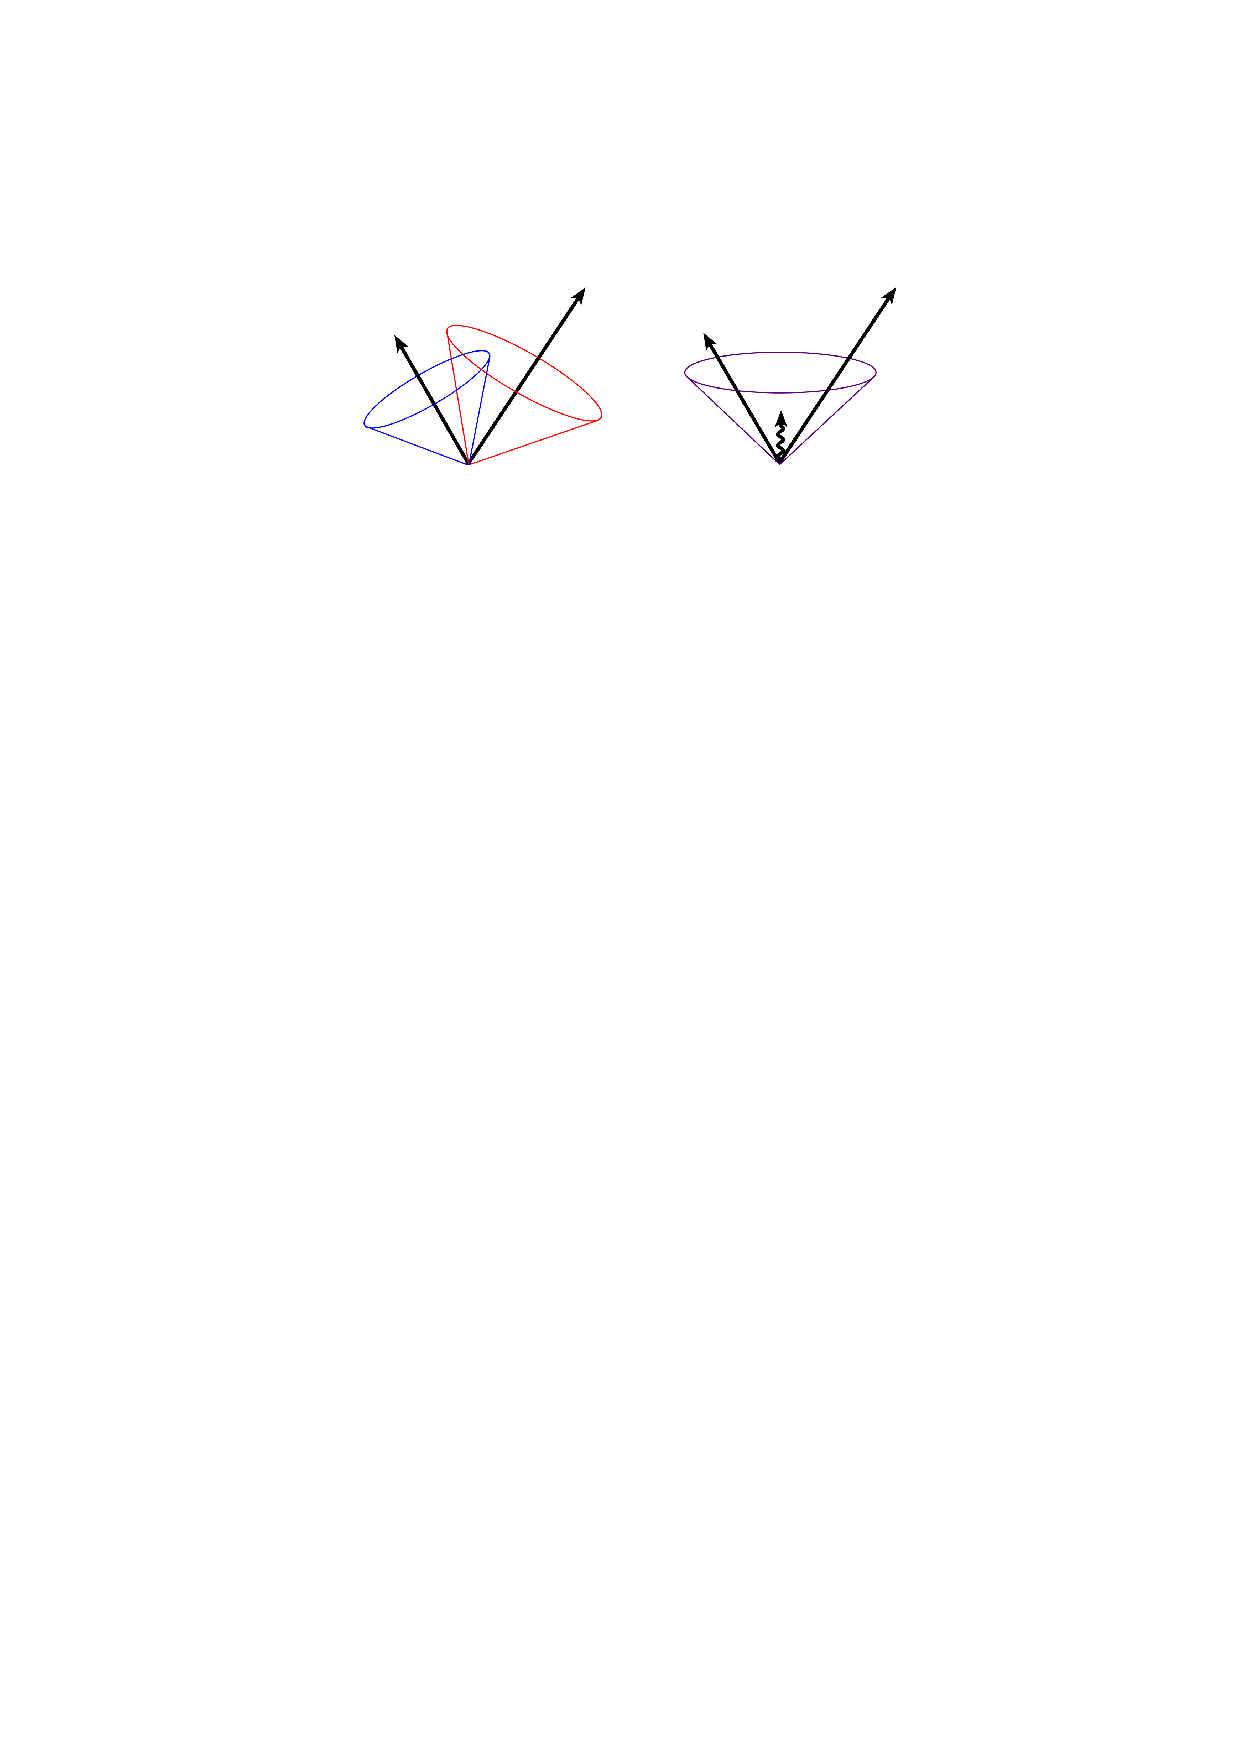
\includegraphics[scale = 1.3]{/home/anter/Desktop/Thesis/Figures/cropped_IR.pdf}\\
%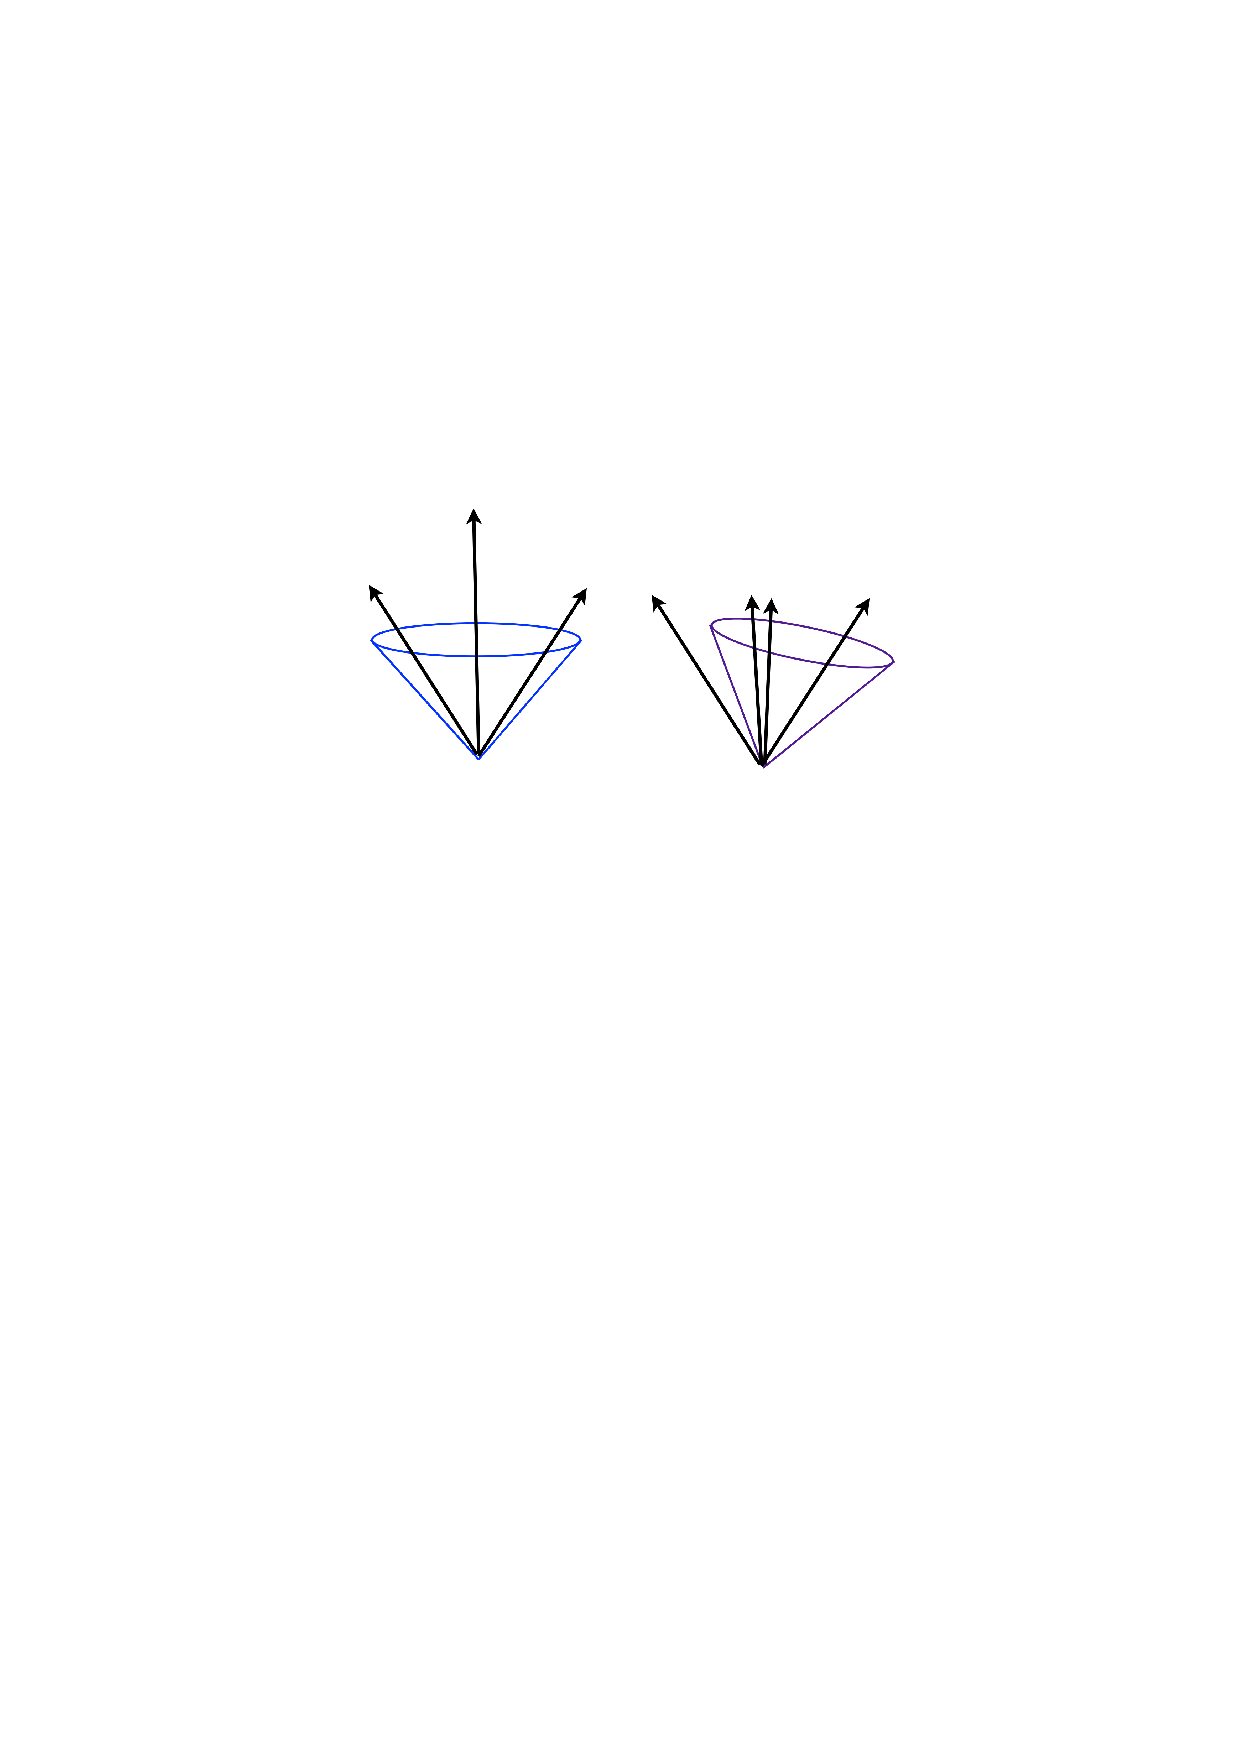
\includegraphics[scale = 1.1]{/home/anter/Desktop/Thesis/Figures/cropped_Collinear.pdf}
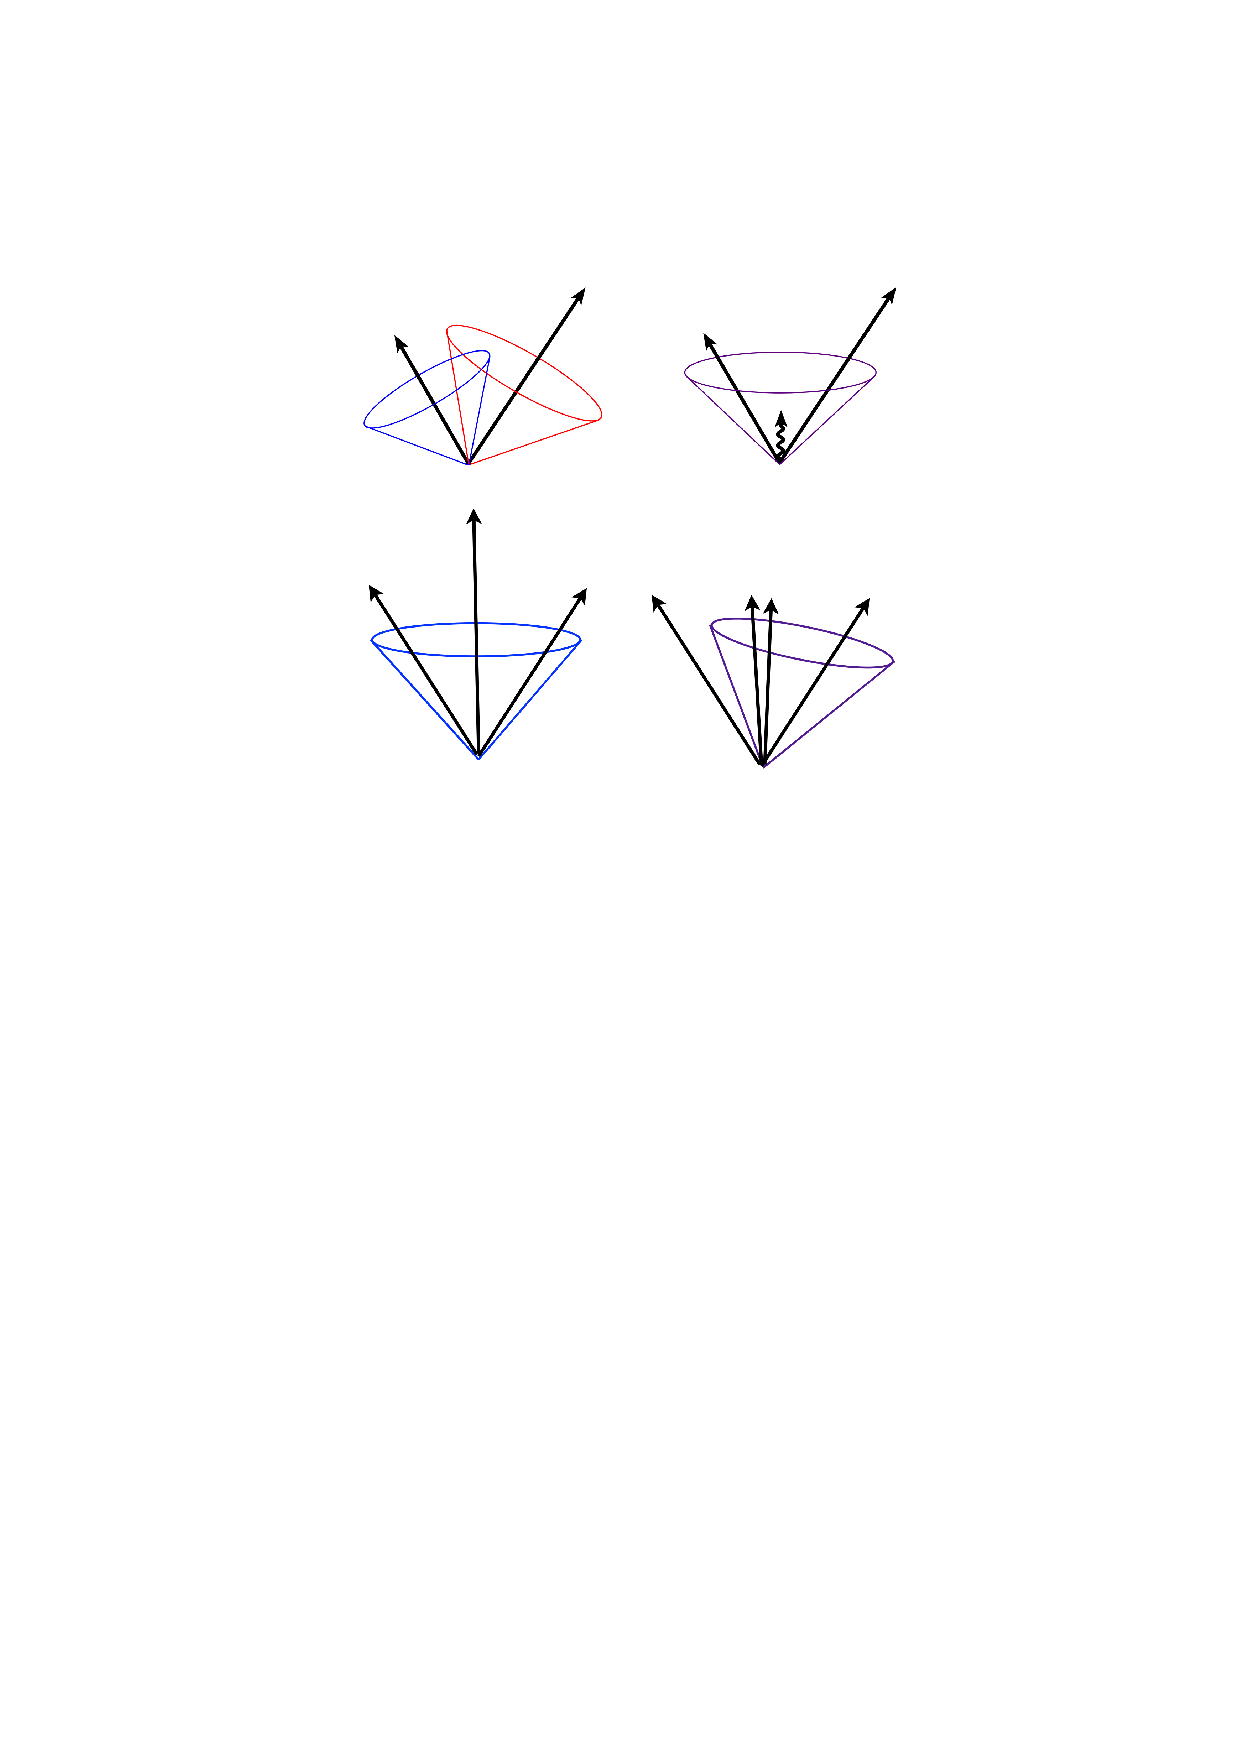
\includegraphics[scale = 0.9]{/home/anter/Desktop/Thesis/Figures/cropped_Algo.pdf}
\caption[Effects of emission of infrared radiations and collinear splitting in jet algorithms.]{Top : Infrared unsafe behavior of jet algorithm is illustrated where the presence of soft radiation between two jets may cause a merging of the jets that would not occur in the absence of the soft radiation. Bottom : Collinear unsafe behavior of jet algorithm is shown in which the number of jets change by a collinear splitting\footnotemark.}
\label{fig:IRC}
\end{center}
\end{figure} 
\footnotetext{Source : \url{http://inspirehep.net/record/1251416}} This can be seen in Fig.~\ref{fig:IRC} (top). Collinear safety is the property by virtue of which the set of hard jets found in the event should not be changed on modification of the event by a collinear splitting i.e. replacement of one parton by two at the same place. The output of the jet algorithm should remain the same if the energy of a particle is distributed among two collinear particles such that the collinear singularities should not appear in the perturbative calculations. It means that two pictures shown in Fig.~\ref{fig:IRC} (bottom) should always produce a single jet. In this case, if an algorithm produces zero or two jets then it is not collinear safe. 

The jet algorithms can be classified mainly into two types : \\ \newline
{\bf Cone algorithms -} In the iterative cone (IC) algorithm \cite{Blazey:2000qt}, the jet is defined as a cone with fixed radius $R$ in $\eta$-$\phi$ space drawn around the highest energy seed. The relative distance of all the particles is iteratively calculated and compared with $R$. If the distance between the considered particles is smaller than $R$, they are clustered together in a jet and the jet direction is updated with the directions of the clustered particles, otherwise they initiate two different jets. The algorithm iterates until the cone is stable which means that the direction of sum of momentum of all the particles is same as that of the center of cone. But IC algorithm is not IRC safe. There is an another cone algorithm, Seedless Infrared-Safe cone (SIS-Cone) \cite{Weinzierl:2011jx}, which is an exact seedless i.e. does not rely on seed threshold and is IRC safe. This is a complex approach which tests the stability of all subsets of particles and has a complexity of ${\cal O}(N2^{N})$ for $N$ particles. But this algorithm is much slower and hence not preferred. \\ \newline
{\bf Sequential algorithms -} The sequential algorithms \cite{Ellis:1993tq} work by defining a distance between pairs of particles and recombining the pair of closest particles successively. This algorithm stops when all the resulting objects are far apart. This is collinear and infrared safe algorithm. It is possible for jet cones to overlap such that one particle is contained in more than one jet but the sequential algorithm never assigns a particle to more than one jet. The procedure for clustering the particles into jets by using sequential algorithm is as follows : 
\begin{enumerate}
\item First the distance $d_{ij}$ between two particles $i$ and $j$ and distance $d_{iB}$ of the particle to the beam are calculated.
 \begin{equation}
\begin{gathered}
d_{ij} = {\rm min}\big(p^{2p}_{{\rm T}i},p^{2p}_{{\rm T}j}\big) \frac{\Delta R^2_{ij}}{R^2}, ~~~~d_{iB} = p^{2p}_{{\rm T}i} \\ {\rm where} ~~~\Delta R^2_{ij} = (\eta_i -\eta_j)^{2} ~\plus (\phi_i -\phi_j)^{2}
\end{gathered}
\end{equation}

\item If $d_{ij}$ \ls $d_{iB}$, then the particles $i$ and $j$ get merged into a new single particle $k$, summing four-momenta of two initial particles by recombination scheme and step 1 is repeated. 
\item If $d_{iB}$ \ls $d_{ij}$, particle $i$ is declared as a final-state jet and the particle gets removed from the list. 
\end{enumerate}
This procedure continues until all particles are clustered into jets. Based on the parameter $p$, there are three important sequential algorithms with distinct properties : $p$ = 1 for the \kt algorithm \cite{Catani:1993hr,Catani:1992zp}, $p$ = 0 for the Cambridge/Aachen algorithm \cite{Dokshitzer:1997in} and $p$ = -1 for the anti-$k_{T}$ algorithm \cite{Cacciari:2008gp}. The \kt algorithm involves clustering of soft particles first resulting in an area that fluctuates considerably. This algorithm is susceptible to the underlying and pile-up events. The C/A algorithm involves energy independent clusterings. Both \kt and C/A produce jets of irregular shapes. Instead of jet analysis, these are widely used for jet substructure studies, where at first a jet with a large jet size is clustered and then its structure is investigated. The anti-$k_{T}$ algorithm tends to cluster hard particles first and produce jets with circular regular shapes. It is less sensitive to underlying and pile-up events. It is the most preferred algorithm for jet studies at the LHC. Figure~\ref{fig:jet_algo} shows the clustering of same particles but using the different jet algorithms. 

\begin{figure}[!h]
\begin{center}
\hspace*{-15mm}
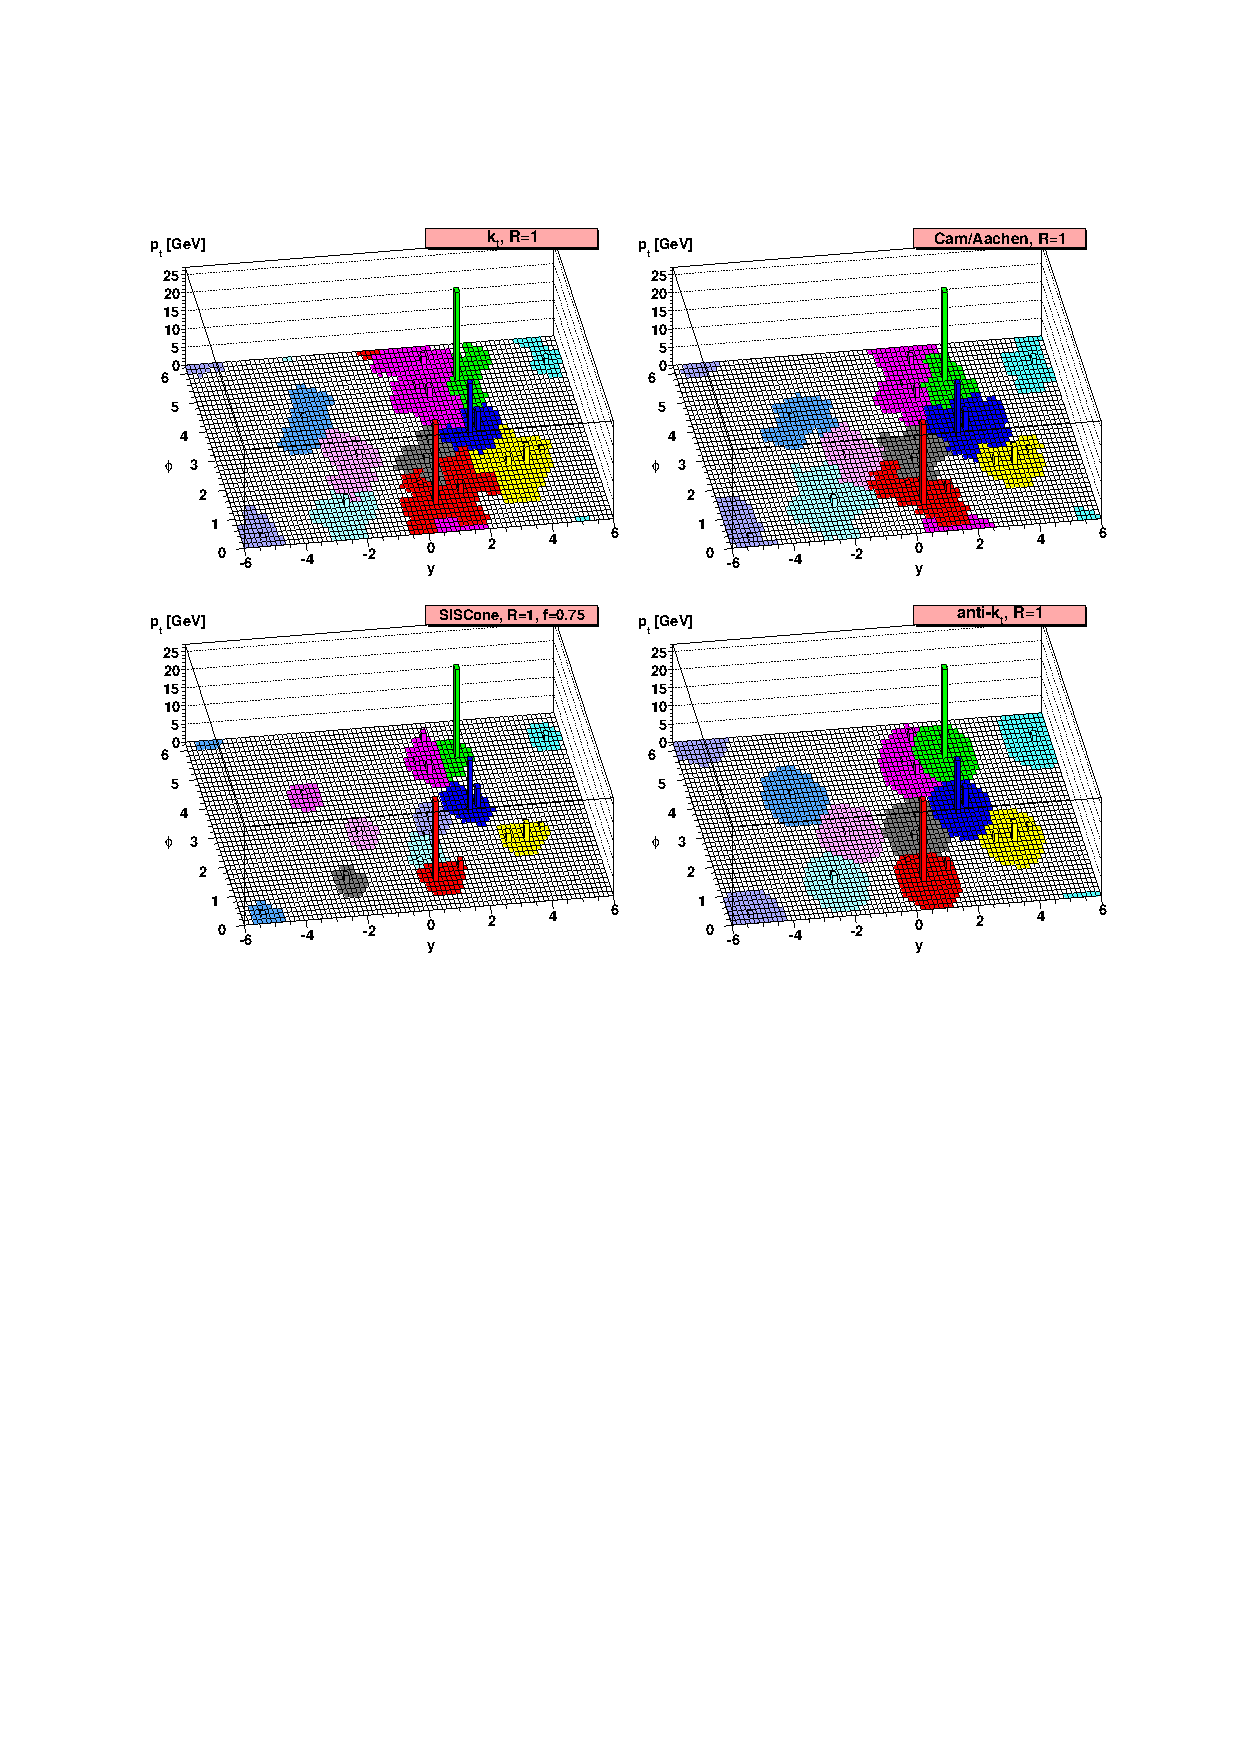
\includegraphics[width=1.2\textwidth]{/home/anter/Desktop/Thesis/Figures/cropped_JetAlgo.pdf}\\
\vspace*{4mm}
\caption[The clustering of particles into jets using different jet algorithms.]{The clustering of particles, in $y$-$\phi$ space at the parton level, into jets clustered with the \kt (top left), Cambridge/Aachen (top right), SISCone (bottom left) and anti-\kt (bottom right) algorithms with $R$ = 1. The towers represent the jet \pt. The anti-\kt algorithm gives circular jets while the jets produced with other algorithms have irregular shapes. Taken from \cite{Salam:2009jx}.}
\label{fig:jet_algo}
\end{center}
\end{figure}

A jet algorithm must specify how to combine the momenta of different partons or particles going to be clustered into a jet. This is given by the recombination scheme. The most widely used recombination scheme is the $E$-scheme \cite{Blazey:2000qt} which corresponds to vector addition of four-momenta i.e. the four-momenta of the jet is obtained by simply adding the four-momenta vector of merging particles.
 
The sequential clustering algorithms have always been favoured by theorists but not by experimentalists because of slow computational performance. However, the introduction of the \fastjet program \cite{Cacciari:2011ma} enhanced the speed of clustering algorithms and hence are preferred by experimentalists as well. This thesis studies the jets clustered, using anti-\kt algorithm with distance parameter $R$ = 0.7, from the particles produced in proton-proton collisions observed in the Compact Muon Solenoid detector of the Large Hadron Collider. The details of the experimental set up are discussed in the coming chapter.
\cleardoublepage
